\section{State of the art}

Quite surprisingly, there is not much work on model-based planning and learning in complex environments, like video games, from images. This chapter researches related work that helps arrive at the final solution of this thesis' problem of planning in imagination.

\subsection{Learning and querying world models}

In this paper \cite{Algo.FastGenerativeModels}, the authors aim to address the challenge of learning accurate, computationally efficient models of complex domains, a key challenge in model-based reinforcement learning, and using them to solve RL problems. First, they advocate the use of computationally efficient state-space environment models that make predictions at a higher level of abstraction, both spatially and temporally, than at the level of raw pixel observations. Such models substantially reduce the amount of computation required to make predictions, as future states can be represented much more compactly. Second, in order to increase model accuracy, they examine the benefits of explicitly modeling uncertainty in state transitions.

In the fig.~\ref{Fig.FastGenerativeModels}, there are different environment models described in the paper. The models, $p$, are learned in an unsupervised way from observations, $o$, conditioned on actions, $a$,. In particular, the authors focus on how fast and accurately models can predict, at time step $t$, some future statistics $x_{t+1:t+\tau}$, e.g. an environment's rewards, over a horizon $\tau$ by doing Monte-Carlo rollouts of the model given an arbitrary sequence of actions $a_{t:t+\tau−1}$, that can later be used for decision making.

\begin{figure}[H]
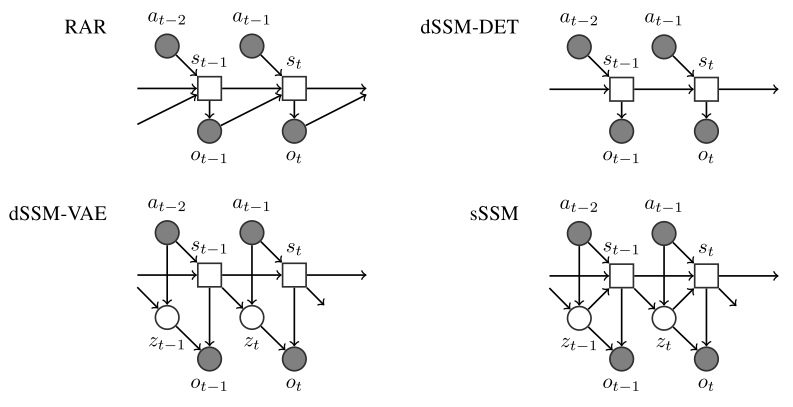
\includegraphics[width=0.9\textwidth,keepaspectratio]{figures/FastGenerativeModels.png}
\caption[Fast Generative Models]{The graphical models representing the architectures of different environment models. Boxes are deterministic nodes, circles are random variables and filled circles represent variables observed during training \protect\cite{Algo.FastGenerativeModels}.}
\label{Fig.FastGenerativeModels}
\end{figure}

A straight-forward choice is the family of temporally auto-regressive models over the observations, $o_{t+1:t+\tau}$. If these use a recurrent mapping that recursively updates sufficient statistics $s_t = f(s_{t−1}, a_{t−1}, o_{t−1})$, therefore reusing the previously computed statistics $s_{t-1}$, and use them to predict future observations, $p(o_{t+1:t+\tau} | o_{\leqslant t}, a_{<t+\tau}) = \prod^{t+\tau}_{r=t+1} p(o_r | f(s_{r−1}, a_{r−1}, o_{r−1}))$, then the authors call these models recurrent auto-regressive models (RAR). If $f$ is parameterised as a neural network, RARs are equivalent to recurrent neural networks. Although faster then auto-regressive models that don't reuse statistics from previous time steps, these are still expect to be slow when generating Monte-Carlo rollouts, as they still need to explicitly render observations $o_{t+1:t+\tau}$ in order to make any predictions, $x_{t+1:t+\tau}$.

State-space models (SSMs) circumvent this by positing that there is a compact state representation $s_t$ that captures all essential aspects of the environment on an abstract level. It is assumed that $s_{t+1}$ can be predicted from the previous state $s_t$ and action $a_t$ alone, without the help of previous pixels $o_{\leqslant t}$, $p(s_{t+1}|s_{\leqslant t}, a_{<t}, o_{\leqslant t}) = p(s_{t+1}| s_t, a_t)$. Furthermore, it is assumed that $s_t$ is sufficient to predict $o_t$, i.e. $p(o_t|s_{\leqslant t}, a_{<t}) = p(o_t|s_t)$. This modelling choice implies that the latent states are, by construction, sufficient to generate any future predictions $x_{t+1:t+\tau}$. Hence, the model never have to directly sample costly high-dimensional pixel observations.

The authors consider two flavors of SSMs: deterministic SSMs (dSSMs) and stochastic SSMs (sSSMs). For dSSMs, the latent transition $s_{t+1} = f(s_t, a_t)$ is a deterministic function of the past, whereas for sSSMs, they consider transition distributions $p(s_{t+1}|s_t, a_t)$ that explicitly model uncertainty over the next state. The sSSMs are parameterised by introducing for every $t$ a latent variable $z_t$ whose distribution depends on $s_{t−1}$ and $a_{t−1}$, and by making the state a deterministic function of the past state, action, and latent variable: $z_{t+1} \sim p(z_{t+1}|s_t, a_t)$, $s_{t+1} = f(s_t, a_t, z_{t+1})$. \\
The observation model computes the conditional distribution $p(o_t|\cdot)$. It either takes as input the state $s_t$ (deterministic decoder), or the state $s_t$ and latent $z_t$ (stochastic decoder). sSSMs always use the stochastic decoder. dSSMs can use either the deterministic decoder (dSSM-DET), or the stochastic decoder (dSSM-VAE). The latter can capture joint uncertainty over pixels in a given observation $o_t$, but not across time steps. The former is a fully deterministic model, incapable of modeling joint uncertainties (in time or in space).

The paper provides the first comparison of deterministic and stochastic, pixel-space and state-space models w.r.t. speed and accuracy, applied to challenging environments from the Arcade Learning Environment \cite{Code.ALE}. Specifically, the prediction of dSSM-DET exhibits “sprite splitting”, or layering of multiple possible future observations, at corridors of MS-PACMAN \cite{Game.MSPACMAN}, whereas multiple samples from the sSSM show that the model has a reasonable and consistent representation of uncertainty in this situation. Moreover, the authors note that SSMs, which avoid computing pixel renderings at each rollout step, exhibit a speedup of more then 5 times over the standard AR model. \\
Extensive experiments establish that state-space models accurately capture the dynamics of Atari games from raw pixels. The computational speed-up of state-space models, while maintaining high accuracy, makes their application in RL feasible. The authors demonstrate that agents which query these models for decision making outperform strong model-free baselines on the game MS-PACMAN, demonstrating the potential of using learned environment models for planning.

The authors explore the topic of learning fast generative models that can be used in model-based reinforcement learning for planning. Their ideas find application in PlaNet \cite{Algo.PlaNet} and World Models \cite{Algo.WorldModels}, the stochastic state-space model (sSSM), and hence in this thesis' solution too.

\subsection{Model-based reinforcement learning}

Model-free reinforcement learning, although can be used to learn effective policies for complex tasks, typically requires very large amounts of data. In fact, substantially more than a human would need to learn the same games. How can people learn so quickly? Part of the answer may be that people can learn how the game works and predict which actions will lead to desirable outcomes. Similar mechanism is used by model-based reinforcement learning. Papers below show a current state of this approach to learning.

\subsubsection{World Models}

In World Models \cite{Algo.WorldModels} paper, its authors explore the idea of using large and highly expressive neural networks, that can learn rich spatial and temporal representation of data, and applying them to reinforcement learning. The RL algorithm is often bottlenecked by the credit assignment problem, which makes it hard for traditional RL algorithms to learn millions of weights of a large model. To accomplish their goal, they decompose the problem of an agent training into two stages: they first train a generative neural network to learn a model of the agent's world in an unsupervised manner. Thereafter, by using a compressed spatial and temporal representation of the environment extracted from the world model as inputs to the agent, they train a linear model to learn to perform a task in the environment. The small linear model lets the training algorithm focus on the credit assignment problem on a small search space, while not scarifying capacity and expressiveness via the larger world model.

Their solution consists of three components: Vision for encoding the spatial information, Memory for encoding the temporal information and Controller which represents the agent's policy. Fig.~\ref{Fig.WorldModels} depicts a flow diagram of the agent's model.

\begin{figure}[H]
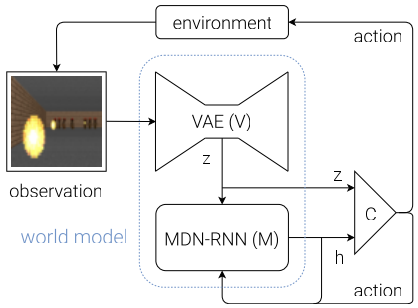
\includegraphics[width=0.7\textwidth,keepaspectratio]{figures/WorldModels.png}
\caption[Flow diagram of the World Models agent's model]{Flow diagram of the agent's model \protect\cite{Algo.WorldModels}. The raw observation is first processed by the Vision at each time step $t$ to produce $z_t$. The input into the Controller is this latent vector $z_t$ concatenated with the Memory hidden state $h_t$ at each time step. The Controller will then output an action vector $a_t$ and will affect the environment. The Memory will then take the current $z_t$ and action $a_t$ as an input to update its own hidden state to produce $h_{t+1}$ to be used at time step $t + 1$.}
\label{Fig.WorldModels}
\end{figure}

The environment provides the agent with a high dimensional visual observation, a game frame, at each time step. The essential task of the Vision model is to encode this high dimensional observation into a low dimensional latent state. To do this, Vision is implemented as Variational Autoencoder \cite{Algo.VAE}. It is trained in an unsupervised manner on randomly generated experience from the environment. The authors assume that the random agent can efficiently explore environment and no iterative training procedure is implemented. The dataset is gathered once and fixed for Vision and Memory training.

Since many complex environment are partially observable, the visual observation at each time step, and hence the latent state, doesn't include full information about the current situation in the environment. To acquire full knowledge, the agent needs to encode what happens over time. This is the role of the Memory. It is implemented as popular recurrent neural network (RNN) architecture called Long Short-Term Memory \cite{Algo.LSTM} and trained on the same data as Vision to predict the next step future latent state that Vision is expected to produce. Because many environments are stochastic in nature, the RNN is trained to output a probability density of the next latent state approximated as a mixture of Gaussian distribution - in literature, this approach is known as Mixture Density Network combined with a RNN \cite{Algo.MDNRNN} (MDN-RNN). Moreover, using the stochastic Memory the authors are able to train more robust Controller, more on that later. \\
To be more precise, the MDN-RNN will model $p(z_{t+1} | o_{\leqslant t}, a_{\leqslant t}) = p(z_{t+1} | h_t) \prod_{i=1}^t q(z_i | o_i)$, where $h_t = f(h_{t-1}, z_t, a_t)$ is the hidden state of the RNN, $f$, that encodes past information about states and actions from the beginning of the episode until the time step $t$. Furthermore, $o_{t}$, $z_{t}$ and $a_{t}$ are the observation, the latent state and the action at time step $t$ respectively. During sampling the authors adjust a temperature parameter $\tau$, that scale mixing coefficients in the MDN, to control model uncertainty \cite{Algo.Sketch-RNN}. They find it useful for training the Controller later on.

The Controller model represents the agent's policy. It is responsible for determining course of actions to take in order to solve a given task. Controller is a simple linear model that maps the concatenated latent state $z_t$ and hidden state $h_t$ at the time step $t$ directly to the action $a_t$ at that time step: $a_t = W[z_t h_t] + b$, where $W$ and $b$ are the weight matrix and bias vector of that model.
The authors deliberately made Controller as simple as possible, and trained it separately from Vision and Memory, so that most of the agent's complexity resides in the world model (Vision and Memory). The latter can take the advantage of current advances in deep learning that provide tools to train large models efficiently when well-behaved and differentiable loss function can be defined.
Shift in the agent's complexity towards the world model allows the Controller model to stay small and focus its training on tackling the credit assignment problem in challenging RL tasks. It is trained using evolution strategy, which is rather an unconventional choice that only currently have been considered as a viable alternative to popular RL techniques \cite{Algo.ESRL}.

Their solution is able to solve an OpenAI Gym's CarRacing environment \cite{Code.OpenAIGym}, which is the continuous-control, top-down racing task. It is the first known solution to achieve the score required to solve this task. Nonetheless, because the Controller uses real experience for training counted in millions of episodes, they did not improve sample-efficiency compared to other model-free solutions \cite{Algo.CarRacingA3C}. But, what is really interesting, in the process of training the Memory learns to simulate the original environment. The authors show that the learned Controller can function inside of the imagined environment of CarRacing, that is, simulated by the Memory.
In the second experiment, they show that the agent can not only play in the imagination, but also it is able to learn solely from imagined experience, produced by its Memory, and successfully transfer this policy back to the actual environment of VizDoom (see fig.~\ref{Fig.VizDoom}). In the first trials, the Controller learned to exploit imperfect simulations of the Model, which only approximates the true environment dynamics. To mitigate this behaviour, they adjust the temperature parameter of MDN-RNN to control the amount of randomness in the Memory, hence controlling the trade-off between realism and exploitability.
The Controller learns from simulated experience, which means that only tens of thousands of episodes from the environment are needed for the training of Vision and Memory. Assuming that each episode consists of hundreds of frames, millions of frames in total are required for training. It makes World Models very sample efficient compared to other state-of-the-art model-free methods that require even two orders of magnitude more data \cite{Algo.A3C}.

\begin{figure}[H]
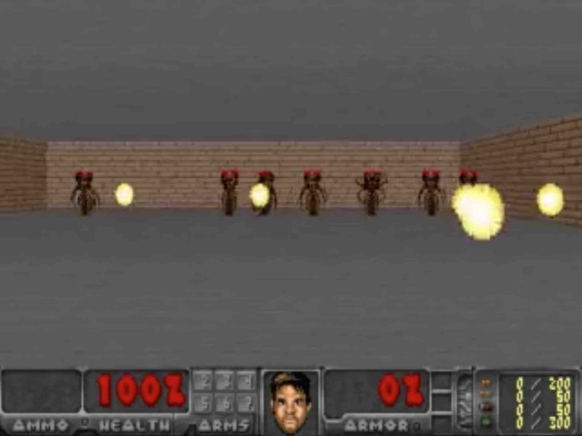
\includegraphics[width=0.7\textwidth,keepaspectratio]{figures/VizDoom.png}
\caption[VizDoom]{VizDoom: the agent must learn to avoid fireballs shot by monsters from the other side of the room with the sole intent of killing the agent \protect\cite{Algo.WorldModels}.}
\label{Fig.VizDoom}
\end{figure}

The authors results indicate that their world model is able to model complex environments from visual observations and it can be used for planning. Therefore, it may prove useful for the topic of this thesis.

\subsubsection{Learning Latent Dynamics for Planning from Pixels}

The authors propose the Deep Planning Network \cite{Algo.PlaNet} (PlaNet), a purely model-based agent that learns the environment dynamics from images and chooses actions through fast online planning in latent space. To achieve high performance, the dynamics model must accurately predict the rewards ahead for multiple time steps. They approach this using a latent dynamics model for its fast querying capabilities. Moreover, they propose a multi-step variational inference objective named latent overshooting.

PlaNet learns a transition model $p(s_t | s_{t-1}, a_{t-1})$, observation model $p(o_t | s_t)$, and reward model $p(r_t | s_t)$ from previously experienced episodes. All of them are Gaussians parameterised by neural networks. The observation model provides a rich training signal but is not used for planning. It also learns an encoder $q(s_t | o_{\leqslant t}, a_{< t})$ to infer an approximate belief over the current hidden state from the history using filtering. This model can be thought of as a non-linear Kalman filter or sequential VAE. The transition model consists of both stochastic and deterministic paths as experiments show that these are crucial for successful planning. \\
Despite its generality, the purely stochastic transitions make it difficult for the transition model to reliably remember information for multiple time steps. In theory, this model could learn to set the variance to zero for some state components, but the optimization procedure may not find this solution. This motivates including a deterministic sequence of activation vectors $\{h_t\}^T_{t=1}$ that allow the model to access not just the last state but all previous states deterministically. The authors use such a model, shown in fig.~\ref{Fig.PlaNetModelDesignes}c, that they name recurrent state-space model (RSSM). Intuitively, one can understand this model as splitting the state into a stochastic part $s_t$ and a deterministic part $h_t$, which depend on the stochastic and deterministic parts at the previous time step through the recurrent neural network (RNN).

\begin{figure}[H]
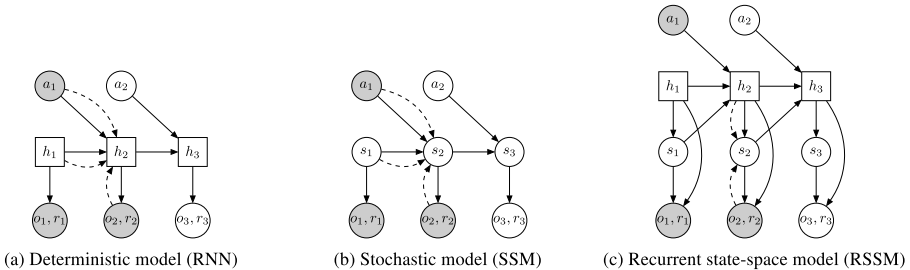
\includegraphics[width=1.0\textwidth,keepaspectratio]{figures/PlaNet/models.png}
\caption[PlaNet latent dynamics model designs]{Latent dynamics model designs \protect\cite{Algo.PlaNet}. In this example, the model observes the first two time steps and predicts the third. Circles represent stochastic variables and squares deterministic variables. Solid lines denote the generative process and dashed lines the inference model. (a) Transitions in a recurrent neural network are purely deterministic. This prevents the model from capturing multiple futures and makes it easy for the planner to exploit inaccuracies. (b) Transitions in a state-space model are purely stochastic. This makes it difficult to remember information over multiple time steps. (c) This model splits the state into stochastic and deterministic parts, allowing the model to robustly learn to predict multiple futures.}
\label{Fig.PlaNetModelDesignes}
\end{figure}

Given these components, the authors implement the policy as a planning algorithm that searches for the best sequence of future actions. In contrast to model-free and hybrid reinforcement learning algorithms, the authors do not use a policy or value network. \\
The cross entropy method \cite{Algo.CEM} (CEM) is used to search for the best action sequence under the model. The authors decided on this algorithm because of its robustness and because it solved all considered tasks when given the true dynamics for planning. CEM is a population-based optimization algorithm that infers a distribution over action sequence that maximize the objective. Starting from zero mean and unit variance time-dependent diagonal Gaussian belief over optimal action sequence up to $H$, the length of the planning horizon, it repeatedly sample $J$ candidate action sequences, evaluate them under the model, and re-fit the belief, mean and variance, to the top best $K$ action sequences. After $I$ iterations, the planner returns the mean of the belief for the current time step. Importantly, after receiving the next observation, the belief over action sequences starts from zero mean and unit variance again to avoid local optima. \\
To evaluate a candidate action sequence under the learned model, PlaNet samples a state trajectory starting from the current state belief and sum the mean rewards predicted along the sequence. Since CEM is a population-based optimizer, the authors found it sufficient to consider a single trajectory per action sequence and thus focus the computational budget on evaluating a larger number of different sequences. Because the reward is modeled as a function of the latent state, the planner can operate purely in latent space without generating images, which allows for fast evaluation of large batches of action sequences.

Since the agent may not initially visit all parts of the environment, it needs to iteratively collect new experience and refine the dynamics model. It does so by planning with the partially trained model. Starting from a small amount of $S$ seed episodes collected under random actions, the authors train the model and add one additional episode to the data set every $C$ update steps.

Typical variational bound for learning and inference in latent sequence models, as show in fig.~\ref{Fig.PlaNetModelUnrolling}a, contains reconstruction terms for the observations and KL-divergence regularisers for the approximate posteriors. A limitation of this objective is that the stochastic path of the transition function $p(s_t | s_{t-1}, a_{t-1})$ is only trained via the KL-divergence regularisers for one-step predictions: the gradient flows through $p(s_t | s_{t-1}, a_{t-1})$ directly into $q(s_{t−1})$ but never traverses a chain of multiple $p(s_t | s_{t-1}, a_{t-1})$. If one could train a model to make perfect one-step predictions, it would also make perfect multi-step predictions, so this would not be a problem. However, when using a model with limited capacity and restricted distributional family, training the model only on one-step predictions until convergence does in general not coincide with the model that is best at multi-step predictions. For successful planning, accurate multi-step predictions are needed. \\
The authors generalize the standard variational bound to latent overshooting, as show in fig.~\ref{Fig.PlaNetModelUnrolling}c, which trains all multi-step predictions in latent space. Using only terms in latent space results in a fast regulariser that can improve long-term predictions, it encourages consistency between one-step and multi-step predictions, and is compatible with any latent sequence model. \\
The authors found that several dynamics models benefit from latent overshooting, although their final agent using the RSSM model does not require it.

\begin{figure}[H]
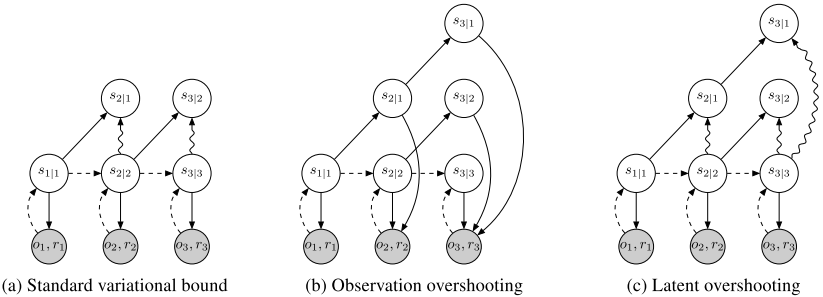
\includegraphics[width=1.0\textwidth,keepaspectratio]{figures/PlaNet/overshooting.png}
\caption[PlaNet latent dynamics model unrolling schemes]{Unrolling schemes \protect\cite{Algo.PlaNet}. The labels $s_{i|j}$ are short for the state at time $i$ conditioned on observations up to time $j$. Arrows pointing at shaded circles indicate log-likelihood loss terms. Wavy arrows indicate KL-divergence loss terms. (a) The standard variational objectives decodes the posterior at every step to compute the reconstruction loss. It also places a KL on the prior and posterior at every step, which trains the transition function for one-step predictions. (b) Observation overshooting decodes all multi-step predictions to apply additional reconstruction losses. This is typically too expensive in image domains. (c) Latent overshooting predicts all multi-step priors. These state beliefs are trained towards their corresponding posteriors in latent space to encourage accurate multi-step predictions.}
\label{Fig.PlaNetModelUnrolling}
\end{figure}

Using only pixel observations, PlaNet's agent solves continuous control tasks from DeepMind control suite (see fig.~\ref{Fig.DeepMindControlSuite}) with contact dynamics, partial observability, and sparse rewards, which exceed the difficulty of tasks that were previously solved by planning with learned models. PlaNet uses substantially fewer episodes and reaches final performance close to and sometimes higher than strong model-free algorithms.

\begin{figure}[H]
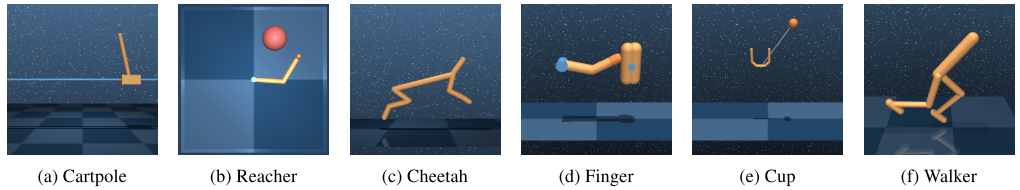
\includegraphics[width=1.0\textwidth,keepaspectratio]{figures/PlaNet/benchmarks.png}
\caption[DeepMind Control Suite]{DeepMind Control Suite: image-based control domains used in PlaNet's experiments \protect\cite{Algo.PlaNet}.}
\label{Fig.DeepMindControlSuite}
\end{figure}

Within 100 episodes, PlaNet outperforms the policy-gradient method A3C \cite{Algo.A3C} trained from proprioceptive states for 100,000 episodes, on all tasks. After 500 episodes, it achieves performance similar to D4PG \cite{Algo.D4PG}, trained from images for 100,000 episodes, except for the finger task. PlaNet surpasses the final performance of D4PG with a relative improvement of 26\% on the cheetah running task.

Moreover, the authors trained a single agent on all six tasks. The agent is not told which task it is facing, it needs to infer this from the image observations. The agent solves all tasks while learning slower compared to individually trained agents. This indicates that the model can learn to predict multiple domains, regardless of the conceptually different visuals.

PlaNet is a working example of a model-based agent that learns a latent dynamics model from high-dimensional image observations and chooses actions by fast planning in latent space. The authors show that their agent succeeds at several continuous control tasks from image observations, reaching performance that is comparable to the best model-free algorithms while using 200 times fewer episodes and similar or less computation time. The results show that learning latent dynamics models for planning in image domains is a promising approach. This thesis will adopt PlaNet to its objectives.

\subsubsection{Model-Based Reinforcement Learning for Atari}

In this paper \cite{Algo.SimPLe}, the authors explore how video prediction models can enable RL agents to solve Atari games with orders of magnitude fewer interactions than model-free methods. They describe Simulated Policy Learning (SimPLe), a complete model-based deep RL algorithm based on video prediction models, and present a comparison of several model architectures, including a novel architecture that yields the best results in Atari setting.

SimPLe, apart from an Atari 2600 emulator environment $env$, use a neural network simulated environment $env'$ which they call a world model. The authors find out that crucial decisions in the design of world models are: inclusion of stochasticity, clipping reconstruction loss to a constant and, because simulator $env'$ is supposed to consume its own predictions from previous steps which will be imperfect due to compounding errors, to mitigate a problem of the model drifting out of the area of its applicability they randomly replace in training some frames of the input by the model prediction from the previous step. 

The environment $env'$ shares the action space and reward space with $env$ and produces visual observations in the same format, as it will be trained to mimic $env$. The authors principal aim is to train a policy $\pi$ using a simulated environment $env'$ so that $\pi$ achieves good performance in the original environment $env$. Using short rollouts for a policy training is crucial to mitigate the compounding errors under the model. To ensure exploration SimPLe starts training rollouts from randomly selected states taken from the real data buffer.

In this training process the authors aim to use as few interactions with $env$ as possible. The initial data to train $env'$ comes from random rollouts of $env$. As this is unlikely to capture all aspects of the environment, they use the data-aggregation iterative method.

Experiments evaluate SimPLe on a range of Atari games and show that it achieves competitive results compared to model-free baselines with only 100K interactions between the agent and the environment, which corresponds to about two hours of real-time play. SimPLe is significantly more sample-efficient than a highly tuned version of the state-of-the-art Rainbow algorithm \cite{Algo.Rainbow} on almost all games. In particular, in low data regime of 100k samples, on more than half of the games, SimPLe achieves a score which Rainbow requires at least twice as many samples. In the best case of Freeway, it is more than 10x more sample-efficient.

SimPLe is a similar approach to model-based RL like in World Models. The authors train the dynamics model and use it to generate new experience, the same as in World Models, but in observations space, opposite to World Models. \\
Although this thesis share the goal of sample efficient RL via model-based planning and learning in complex environments, like Atari games, with SimPLe, it tries to accomplish it in fundamentally different way. The thesis' solution focuses on train accurate transitions model in the latent state-space to enable fast simulation and search using this model. Pixel-perfect reconstructions are not a concern.

\subsection{Monte-Carlo planning}

Planning is a natural and powerful approach to decision making problems with known dynamics. For instance, Monte-Carlo Tree Search methods \cite{Algo.MCTS} have been used for complex search problems, such as the game of Go \cite{Algo.AlphaGoZero}. Moreover, planning carries the promise of increasing performance just by increasing the computational budget for searching for actions. The first paper below describes current state of the art search method and the other one explores the idea of Monte-Carlo planning with a learned model.

\subsubsection{A general reinforcement learning algorithm that masters chess, shogi, and Go}

AlphaZero \cite{Algo.AlphaZero} replaces the handcrafted knowledge and domain-specific augmentations used in traditional game-playing programs with deep neural networks, a general-purpose reinforcement learning algorithm, and a general-purpose tree search algorithm. Instead of handcrafted move ordering and evaluation function heuristics, AlphaZero infers policy and state value with a deep neural network. This neural network takes the board position as an input and outputs a vector of move probabilities for each action and a scalar value estimating the expected outcome of the game. AlphaZero learns these move probabilities and value estimates entirely from self-play. These are then used to guide its search in future games.

Instead of an alpha-beta search with domain-specific enhancements, as common in board games playing programs, AlphaZero uses a general-purpose Monte Carlo tree search \cite{Algo.MCTS} algorithm. Each search consists of a series of simulated games that traverse a tree from a root state until a leaf state is reached. Each simulation proceeds by selecting in each state a move with low visit count (not previously frequently explored), high move probability and high value (averaged over the leaf states of simulations that selected this move previously) according to the current neural network. The search returns a vector representing a probability distribution over moves from the root state. \\
The parameters of the deep neural network in AlphaZero are trained by reinforcement learning from self-play games, starting from randomly initialized parameters. Each game is played by running the search, described above, from the current position and then selecting a move either proportionally (for exploration) or greedily (for exploitation) according to returned move probabilities, which are normalised visit counts at the root state. At the end of the game, the terminal position is scored according to the rules of the game to compute the game outcome: −1 for a loss, 0 for a draw, and +1 for a win. The neural network parameters are updated to minimize the error between the predicted outcome and the game outcome, and to maximize the similarity of the predicted move probabilities to the search probabilities. The updated parameters are used in subsequent games of self-play.

Starting from random play, AlphaZero convincingly defeats a world champion programs in the games of chess and shogi as well as Go. Especially, the game of chess represents the pinnacle of artificial intelligence research over several decades. State-of-the-art programs are based on powerful engines that search many millions of positions, leveraging handcrafted domain expertise and sophisticated domain adaptations. AlphaZero is a generic reinforcement learning and search algorithm, originally devised for the game of Go, that achieve superior results within a few hours, searching 1/1000 as many positions and it is given no domain knowledge except the rules of chess. Furthermore, the same algorithm was applied without modification to the more challenging game of shogi, again outperforming state-of-the-art programs within a few hours.

AlphaZero is the state-of-the-art general search algorithm, but it requires a dynamics model of an environment in order to work. The model is not always available, but could be learned in such cases. This thesis tries to enable AlphaZero to work with the learned model. This work is described in the next chapters.

\subsubsection{Value Prediction Network}

This paper \cite{Algo.VPN} proposes a novel deep reinforcement learning architecture, called Value Prediction Network (VPN), which integrates model-based (i.e. learning an abstract dynamics model) and model-free (i.e. mapping the learned abstract states to rewards and values) RL methods into a single neural network. In contrast to typical model-based RL methods, VPN learns the dynamics model of an abstract state space sufficient for predicting future rewards and values, rather than future observations. \\
In order to train VPN, the authors propose a combination of temporal-difference search \cite{Algo.TDSearch} and n-step Q-learning \cite{Algo.A3C}. In brief, VPN learns to predict values via Q-learning and rewards via supervised learning. At the same time, VPN perform lookahead planning to choose actions and compute bootstrapped target Q-values.

VPN has the ability to simulate the future and plan based on the simulated future abstract-states. Although many existing planning methods (e.g. MCTS) can be applied to the VPN, the authors implement a simple planning method which performs Monte-Carlo rollouts using the VPN up to a certain depth and aggregates all intermediate value estimates as described in the paper \cite{Algo.VPN}. The planning procedure estimates the current state Q-values which an agent uses to decide on the next action.

Experimental results show that VPN has several advantages over both model-free and model-based baselines in a stochastic navigation task where careful planning is required but building an accurate observation-prediction model is difficult. Furthermore, VPN outperforms Deep Q-Network \cite{Algo.DQN}, strong model-free baseline method, on several Atari games even with short-lookahead planning, demonstrating its potential as a new way of learning a good state representation.

VPN uses an abstract model of rewards to augment model-free learning with good results on a number of Atari games. However, this method does not actually aim to model or predict future environment's states and achieves clear but relatively modest gains in sample-efficiency. On the other hand, it is an example of simple tree search algorithm which can successfully use the learned model for planning, something that this thesis could base on.
